\section{Results} 

%\subsection{Overall Performance of Methods}

\begin{table*}[ht!]
  \caption{Overall Performance of the Tested Sentiment Analysis Approaches}\label{tab:performance}
\footnotesize
\begin{tabularx}{\textwidth}{lXXrrrrrrrr}
\toprule
& & & & & \multicolumn{3}{c}{Positive} & \multicolumn{3}{c}{Negative} \\
\cmidrule(r){6-8}\cmidrule(l){9-11} 
\multicolumn{3}{l}{Method} & Acc. & $\alpha$ & Pr. & Re. & F1& Pr. & Re. & F1 \\
\midrule

\multicolumn{11}{l}{\emph{ Manual Coding }} \\

 & \multicolumn{2}{l}{ Single Coder }& \cellcolor[gray]{0.59} 0.82& \cellcolor[gray]{0.59} 0.82& \cellcolor[gray]{0.56} 0.88& \cellcolor[gray]{0.57} 0.86& \cellcolor[gray]{0.57} 0.87& \cellcolor[gray]{0.58} 0.84& \cellcolor[gray]{0.60} 0.80& \cellcolor[gray]{0.59} 0.82\\

 & \multicolumn{2}{l}{ Vote (3 Coders) }& \cellcolor[gray]{0.56} 0.88& \cellcolor[gray]{0.55} 0.90& \cellcolor[gray]{0.52} 0.97& \cellcolor[gray]{0.54} 0.91& \cellcolor[gray]{0.53} 0.94& \cellcolor[gray]{0.56} 0.87& \cellcolor[gray]{0.58} 0.84& \cellcolor[gray]{0.57} 0.86\\


\multicolumn{11}{l}{\emph{ Crowd-Coding }} \\

 & \multicolumn{2}{l}{ Single Coder }& \cellcolor[gray]{0.64} 0.72& \cellcolor[gray]{0.62} 0.75& \cellcolor[gray]{0.65} 0.69& \cellcolor[gray]{0.58} 0.84& \cellcolor[gray]{0.62} 0.76& \cellcolor[gray]{0.61} 0.78& \cellcolor[gray]{0.61} 0.78& \cellcolor[gray]{0.61} 0.78\\

 & \multicolumn{2}{l}{ Vote (3 Coders) }& \cellcolor[gray]{0.62} 0.77& \cellcolor[gray]{0.60} 0.81& \cellcolor[gray]{0.63} 0.73& \cellcolor[gray]{0.55} 0.89& \cellcolor[gray]{0.60} 0.80& \cellcolor[gray]{0.58} 0.83& \cellcolor[gray]{0.59} 0.81& \cellcolor[gray]{0.59} 0.82\\

 & \multicolumn{2}{l}{ Vote (5 Coders) }& \cellcolor[gray]{0.62} 0.77& \cellcolor[gray]{0.59} 0.81& \cellcolor[gray]{0.63} 0.73& \cellcolor[gray]{0.55} 0.90& \cellcolor[gray]{0.60} 0.81& \cellcolor[gray]{0.58} 0.84& \cellcolor[gray]{0.60} 0.80& \cellcolor[gray]{0.59} 0.82\\


\multicolumn{11}{l}{\emph{ Machine Learning }} \\

 & \multicolumn{2}{l}{ CNN }& \cellcolor[gray]{0.68} 0.63& \cellcolor[gray]{0.75} 0.50& \cellcolor[gray]{0.66} 0.68& \cellcolor[gray]{0.76} 0.49& \cellcolor[gray]{0.72} 0.56& \cellcolor[gray]{0.64} 0.72& \cellcolor[gray]{0.71} 0.57& \cellcolor[gray]{0.68} 0.63\\

 & \multicolumn{2}{l}{ SVM }& \cellcolor[gray]{0.71} 0.58& \cellcolor[gray]{0.79} 0.42& \cellcolor[gray]{0.65} 0.70& \cellcolor[gray]{0.81} 0.38& \cellcolor[gray]{0.75} 0.50& \cellcolor[gray]{0.68} 0.64& \cellcolor[gray]{0.75} 0.49& \cellcolor[gray]{0.72} 0.56\\


\multicolumn{11}{l}{\emph{ Dictionaries }} \\

 & \multicolumn{2}{l}{ DANEW }& \cellcolor[gray]{0.79} 0.42& \cellcolor[gray]{0.95} 0.10& \cellcolor[gray]{0.62} 0.75& \cellcolor[gray]{0.96} 0.08& \cellcolor[gray]{0.93} 0.15& \cellcolor[gray]{0.60} 0.80& \cellcolor[gray]{0.98} 0.04& \cellcolor[gray]{0.96} 0.08\\

 & \multicolumn{2}{l}{ DamstraBoukes }& \cellcolor[gray]{0.80} 0.41& \cellcolor[gray]{0.97} 0.05& \cellcolor[gray]{0.58} 0.83& \cellcolor[gray]{0.97} 0.07& \cellcolor[gray]{0.94} 0.13& \cellcolor[gray]{1.00} 0.00& \cellcolor[gray]{1.00} 0.00& \cellcolor[gray]{1.00} 0.00\\

 & \multicolumn{2}{l}{ Muddiman }& \cellcolor[gray]{0.76} 0.49& \cellcolor[gray]{0.84} 0.31& \cellcolor[gray]{0.74} 0.53& \cellcolor[gray]{0.81} 0.38& \cellcolor[gray]{0.78} 0.44& \cellcolor[gray]{0.73} 0.53& \cellcolor[gray]{0.80} 0.39& \cellcolor[gray]{0.77} 0.45\\

 & \multicolumn{2}{l}{ NRC }& \cellcolor[gray]{0.76} 0.47& \cellcolor[gray]{0.84} 0.32& \cellcolor[gray]{0.80} 0.39& \cellcolor[gray]{0.73} 0.53& \cellcolor[gray]{0.77} 0.45& \cellcolor[gray]{0.71} 0.59& \cellcolor[gray]{0.77} 0.46& \cellcolor[gray]{0.74} 0.52\\

 & \multicolumn{2}{l}{ Pattern }& \cellcolor[gray]{0.81} 0.39& \cellcolor[gray]{0.97} 0.07& \cellcolor[gray]{0.79} 0.43& \cellcolor[gray]{0.96} 0.08& \cellcolor[gray]{0.93} 0.14& \cellcolor[gray]{0.81} 0.38& \cellcolor[gray]{0.98} 0.03& \cellcolor[gray]{0.97} 0.06\\

 & \multicolumn{2}{l}{ Polyglot }& \cellcolor[gray]{0.79} 0.42& \cellcolor[gray]{0.87} 0.26& \cellcolor[gray]{0.81} 0.38& \cellcolor[gray]{0.84} 0.32& \cellcolor[gray]{0.83} 0.34& \cellcolor[gray]{0.73} 0.53& \cellcolor[gray]{0.83} 0.33& \cellcolor[gray]{0.80} 0.41\\


\multicolumn{11}{l}{\emph{ English Dictionaries (translated using deepl) }} \\

 & \multicolumn{2}{l}{ AFINN }& \cellcolor[gray]{0.79} 0.43& \cellcolor[gray]{0.86} 0.27& \cellcolor[gray]{0.82} 0.35& \cellcolor[gray]{0.81} 0.38& \cellcolor[gray]{0.82} 0.37& \cellcolor[gray]{0.71} 0.58& \cellcolor[gray]{0.81} 0.38& \cellcolor[gray]{0.77} 0.46\\

 & \multicolumn{2}{l}{ DamstraBoukes }& \cellcolor[gray]{0.79} 0.42& \cellcolor[gray]{0.96} 0.07& \cellcolor[gray]{0.67} 0.67& \cellcolor[gray]{0.96} 0.08& \cellcolor[gray]{0.93} 0.15& \cellcolor[gray]{0.50} 1.00& \cellcolor[gray]{0.99} 0.02& \cellcolor[gray]{0.98} 0.04\\

 & \multicolumn{2}{l}{ GenInq }& \cellcolor[gray]{0.80} 0.41& \cellcolor[gray]{0.87} 0.26& \cellcolor[gray]{0.84} 0.31& \cellcolor[gray]{0.82} 0.37& \cellcolor[gray]{0.83} 0.34& \cellcolor[gray]{0.73} 0.54& \cellcolor[gray]{0.76} 0.47& \cellcolor[gray]{0.75} 0.51\\

 & \multicolumn{2}{l}{ HuLiu }& \cellcolor[gray]{0.77} 0.46& \cellcolor[gray]{0.83} 0.34& \cellcolor[gray]{0.80} 0.40& \cellcolor[gray]{0.85} 0.30& \cellcolor[gray]{0.83} 0.34& \cellcolor[gray]{0.68} 0.65& \cellcolor[gray]{0.80} 0.40& \cellcolor[gray]{0.75} 0.50\\

 & \multicolumn{2}{l}{ LoughranMcDonald }& \cellcolor[gray]{0.75} 0.50& \cellcolor[gray]{0.85} 0.29& \cellcolor[gray]{0.75} 0.50& \cellcolor[gray]{0.93} 0.14& \cellcolor[gray]{0.89} 0.22& \cellcolor[gray]{0.69} 0.62& \cellcolor[gray]{0.78} 0.43& \cellcolor[gray]{0.74} 0.51\\

 & \multicolumn{2}{l}{ LSD }& \cellcolor[gray]{0.77} 0.46& \cellcolor[gray]{0.84} 0.33& \cellcolor[gray]{0.80} 0.39& \cellcolor[gray]{0.80} 0.40& \cellcolor[gray]{0.80} 0.39& \cellcolor[gray]{0.69} 0.62& \cellcolor[gray]{0.79} 0.41& \cellcolor[gray]{0.75} 0.50\\

 & \multicolumn{2}{l}{ Muddiman }& \cellcolor[gray]{0.76} 0.48& \cellcolor[gray]{0.87} 0.27& \cellcolor[gray]{0.76} 0.48& \cellcolor[gray]{0.81} 0.38& \cellcolor[gray]{0.79} 0.43& \cellcolor[gray]{0.72} 0.57& \cellcolor[gray]{0.85} 0.30& \cellcolor[gray]{0.80} 0.39\\

 & \multicolumn{2}{l}{ NRC }& \cellcolor[gray]{0.79} 0.42& \cellcolor[gray]{0.89} 0.23& \cellcolor[gray]{0.83} 0.34& \cellcolor[gray]{0.69} 0.62& \cellcolor[gray]{0.78} 0.44& \cellcolor[gray]{0.72} 0.57& \cellcolor[gray]{0.80} 0.39& \cellcolor[gray]{0.77} 0.46\\

 & \multicolumn{2}{l}{ RID }& \cellcolor[gray]{0.79} 0.42& \cellcolor[gray]{0.97} 0.06& \cellcolor[gray]{1.00} 0.00& \cellcolor[gray]{1.00} 0.00& \cellcolor[gray]{1.00} 0.00& \cellcolor[gray]{0.59} 0.82& \cellcolor[gray]{0.95} 0.09& \cellcolor[gray]{0.92} 0.16\\


\bottomrule
\end{tabularx}


\emph{Note}: Acc.: Accuracy expressed as percentage correct; $\alpha$: Krippendorff's alpha (ordinal), Pr.: Precision for the specified class (Positive/Neutral/Negative); Re.: Recall for that class; F1: F1-Score for that class.\\ When more than one measurement or prediction (respectively for manual/ crowd annotation and machine learning) was available, we averaged the score.
\end{table*}

\noindent Table \ref{tab:performance} shows the overall performance of all tested methods, listed as percentage agreement (\textsf{acc}), Krippendorff's $\alpha$ for ordinal measures, as well as the precision, recall, and F1 score for both positive, neutral, and negative sentiment.% 
\footnote{See the online compendium for all code and materials used in this article. For review, an anonymous version of this compendium is available here: \url{https://anonymous.4open.science/r/475de8a9-6796-4538-95bc-94182a2e5557/}}
These latter scores are given since they are the standard for performance evaluation in machine learning, 
but they also give more insight into the type of error made by an algorithm.
For example, a dictionary with only a few very clear sentiment words can have high precision but low recall,
meaning that when it identifies a document as positive or negative it is generally correct (precision),
but that it misses a lot of the documents that were actually positive or negative (recall) 
because these documents did not contain the words in the dictionary. 
The F1 score is the harmonic mean between precision and recall and will generally be closest to the lower of the two scores. 
Since Krippendorff's $\alpha$ is the most commonly used measure for the validity of text analysis in communication science,
we will mostly report performance using that measure, but overall accuracy, $\alpha$, and F1 scores show the same pattern for all cases. 

Starting with the top rows of Table~\ref{tab:performance}, manual coding (using undergraduate students) yields the best results,
with both accuracy and alpha above .8. 
Particularly, using three different students as manual annotators in combination with a majority vote to determine the final sentiment of the sentence achieves the highest performance scores, although this is of course expensive for large scale projects.

A good second place is taken by crowd coding -- rows 3 to 5 in Table~\ref{tab:performance}.
Using just one crowd coder already yields a reasonably good performance ($\alpha\geq0.75$).
This can be further improved by applying a majority vote decision when using multiple crowd coders (an increase to $\alpha\geq0.8$).

Moving from manual annotation to the realm where `computers do the work', Table~\ref{tab:performance} demonstrates that machine learning performs worse than both students' manual coding and crowd coding.
Reaching $\alpha=0.50$ for deep learning (CNN) and slightly worse for classical machine learning (SVM; $\alpha=0.41$, NB; $\alpha=0.40$),
machine learning still performs significantly better than chance. 
However, since these results are lower than generally accepted levels of inter-coder reliability, these models cannot directly be used for substantive analyses.

Finally, the bottom half of Table \ref{tab:performance} shows the performance of Dutch dictionaries and English dictionaries applied to machine translated texts.
These methods perform worse than the machine learning results and much worse than manual annotation.
Most overall performance scores of the dictionaries approximate chance agreement for three categories (i.e. positive, negative and neutral).
Ultimately,  \cite{hu2004} scores best on inter-coder reliability ($\alpha=0.34$), although \cite{loughran2011} does better when considering percentage agreement ($50\%$), possibly because it is more prone to confuse positive and negative, which is penalized more than confusing with neutral in Krippendorff's ordinal measurement. 

Some dictionaries seem reasonably able to measure both positive and negative sentiment looking at the precision scores -- e.g. the custom made dictionary of \cite{damstra2018} reaches a precision score of $0.83$ for positivity, and \cite{martindale1975, martindale1992}'s RID reach equally high levels of precision for negativity. 
The low levels of performance of dictionaries stems from extremely low scores on the recall measure.
Thus, relying on these dictionaries yields many \emph{false negative} cases, also referred to as type II errors. 

\subsection{Trade-off between Coverage and Accuracy}
\begin{figure*}[ht!]
\caption{Coverage vs Accuracy for Crowd Coding and Machine Learning}\label{fig:crowd}
\fitfigure[width=.8\textwidth]{figures/fig_coverage.pdf}

{\small \textit{Note:} For \emph{Machine Learning} (CNN and SVM), points show the percentage accuracy on the subset of documents on which the algorithm was most confident. 
For example, the second dash-dotted triangle shows that the CNN model was accurate in about 84\% of cases for the 20\% of documents on which it was most confident.
For \emph{Crowd Coding}, the lines indicate how many coders were used, and each point represents a majority vote of at least that size. 
For example, the point `4/5' shows that if at least 4 out of 5 coders agreed on a label, they were correct in almost 90\% of cases (accuracy), 
but only just under 75\% of documents were coded with this majority (coverage).}
\end{figure*}

\noindent As explained above, crowd coding using multiple coders achieved results that are very close to coding by trained students,
presenting researchers with a more affordable option. 
This raises the question of how many crowd coders should code each article?
To answer this question, Figure~\ref{fig:crowd} shows the relation between performance in percentage accuracy and coverage, i.e. what percentage of all articles can be coded at a certain reliability. 
The highest point of the solid line ($5/5$) indicates that five out of five crowd coders agreed on approximately 40\% of the sentences (i.e. coverage).
In this case, the coders achieved an accuracy of $>97\%$, or near-perfect coding. 
Utilizing three coders and having them all agree ($3/3$) leads to $93\%$ accuracy for over half of the sentences -- i.e. coverage $>50\%$. 
Hence, when all three coders agree, the researcher can be very confident that the score is correct. 
Looking at the majority-vote scenario -- i.e. $4/5$, $3/5$, or $2/3$ -- Figure \ref{fig:crowd} presents an increase in coverage: From 75\% in a $4/5$ scenario to almost 100\% coverage using $3/5$, or $2/3$.
The performance varies between just under $90\%$ and $75\%$ for the respective majority vote scenarios. 

The results of Figure~\ref{fig:crowd} suggest that the best strategy is to code all texts with two coders initially, and use a third coder on the $<30\%$ of sentences that they disagree on. 
Besides giving a high overall validity, this also gives some measure of which texts were more difficult to code, 
giving an indication of the ambiguity of the sentiment in these texts. 
Adding more coders (up to the five tested here) does not significantly increase overall performance, but does give a better idea of the spread or uncertainty of the annotations, as sentences on which 4 out of 5 agree score significantly better than the ones on which only 3 out of 5 agree, and sentences on which all 5 coders agree are almost certain to be correct. 

The bottom lines of Figure~\ref{fig:crowd} show a similar trade-off for machine learning. 
Where the size of the majority vote in crowd coding gives an indication of the uncertainty of the coded sentiment,
machine learning models give a \emph{confidence} score for each prediction.
Thus, we can choose to use only the predictions on which the algorithm was sufficiently confident, 
and for example use manual coding for the more difficult sentences. 
As shown in the figure, an accuracy of almost $80\%$ can be achieved by CNN for the 30\% of cases on which is was most confident,
and on the 50\% of cases it scored just under $70\%$.

\subsection{Correlation between Various Dictionaries}
\begin{table*}[ht!]
  \caption{Bi-variate Correlations between Dictionaries and Gold Standard}\label{tab:corr}
\newcommand{\squeeze}[1]{$\!\!\!\!$#1$\!\!\!$}
\newcommand{\sectbreak}[1]{$\!\!\!$}
\begin{tabularx}{\textwidth}{lXlclllllllllllllll}
\toprule

& $\!\!\!\!\!$& \squeeze{ Gold }
& $\!\!\!\!\!$& \squeeze{ D1 }& \squeeze{ D2 }& \squeeze{ D3 }& \squeeze{ D4 }& \squeeze{ D5 }& \squeeze{ D6 }
& $\!\!\!\!\!$& \squeeze{ E1 }& \squeeze{ E2 }& \squeeze{ E3 }& \squeeze{ E4 }& \squeeze{ E5 }& \squeeze{ E6 }& \squeeze{ E7 }& \squeeze{ E8 }
\\
\midrule




 
\multicolumn{10}{l}{\emph{ Dictionaries }} \\
& D1: DANEW&\cellcolor[gray]{0.88}
 \squeeze{ .22 } &\sectbreak\ &&&&&& &\sectbreak\ &&&&&&&&\\
& D2: DamstraBoukes&\cellcolor[gray]{0.90}
 \squeeze{ .18 } &\sectbreak\ &\cellcolor[gray]{0.94}
 \squeeze{ .11 }&&&&& &\sectbreak\ &&&&&&&&\\
& D3: Muddiman&\cellcolor[gray]{0.83}
 \squeeze{ .32 } &\sectbreak\ &\cellcolor[gray]{0.88}
 \squeeze{ .23 }&\cellcolor[gray]{0.87}
 \squeeze{ .24 }&&&& &\sectbreak\ &&&&&&&&\\
& D4: NRC&\cellcolor[gray]{0.83}
 \squeeze{ .33 } &\sectbreak\ &\cellcolor[gray]{0.88}
 \squeeze{ .23 }&\cellcolor[gray]{0.94}
 \squeeze{ .11 }&\cellcolor[gray]{0.79}
 \squeeze{ .40 }&&& &\sectbreak\ &&&&&&&&\\
& D5: Pattern&\cellcolor[gray]{0.93}
 \squeeze{ .12 } &\sectbreak\ &\cellcolor[gray]{0.90}
 \squeeze{ .17 }&\cellcolor[gray]{1.00}
 \squeeze{ .00 }&\cellcolor[gray]{0.96}
 \squeeze{ .07 }&\cellcolor[gray]{0.91}
 \squeeze{ .17 }&& &\sectbreak\ &&&&&&&&\\
& D6: Polyglot&\cellcolor[gray]{0.86}
 \squeeze{ .27 } &\sectbreak\ &\cellcolor[gray]{0.90}
 \squeeze{ .18 }&\cellcolor[gray]{0.93}
 \squeeze{ .11 }&\cellcolor[gray]{0.89}
 \squeeze{ .20 }&\cellcolor[gray]{0.82}
 \squeeze{ .35 }&\cellcolor[gray]{0.88}
 \squeeze{ .21 }& &\sectbreak\ &&&&&&&&\\




 
\multicolumn{10}{l}{\emph{ English Dictionaries (translated using deepl) }} \\
& E1: AFINN&\cellcolor[gray]{0.85}
 \squeeze{ .28 } &\sectbreak\ &\cellcolor[gray]{0.89}
 \squeeze{ .20 }&\cellcolor[gray]{0.96}
 \squeeze{ .06 }&\cellcolor[gray]{0.79}
 \squeeze{ .40 }&\cellcolor[gray]{0.84}
 \squeeze{ .31 }&\cellcolor[gray]{0.90}
 \squeeze{ .17 }&\cellcolor[gray]{0.86}
 \squeeze{ .26 } &\sectbreak\ &&&&&&&&\\
& E2: DamstraBoukes&\cellcolor[gray]{0.90}
 \squeeze{ .18 } &\sectbreak\ &\cellcolor[gray]{0.95}
 \squeeze{ .08 }&\cellcolor[gray]{0.69}
 \squeeze{ .61 }&\cellcolor[gray]{0.90}
 \squeeze{ .18 }&\cellcolor[gray]{0.94}
 \squeeze{ .10 }&\cellcolor[gray]{0.99}
 \squeeze{ .00 }&\cellcolor[gray]{0.98}
 \squeeze{ .03 } &\sectbreak\ &\cellcolor[gray]{0.93}
 \squeeze{ .12 }&&&&&&&\\
& E3: GenInq&\cellcolor[gray]{0.86}
 \squeeze{ .26 } &\sectbreak\ &\cellcolor[gray]{0.88}
 \squeeze{ .21 }&\cellcolor[gray]{0.97}
 \squeeze{ .03 }&\cellcolor[gray]{0.84}
 \squeeze{ .30 }&\cellcolor[gray]{0.88}
 \squeeze{ .23 }&\cellcolor[gray]{0.91}
 \squeeze{ .16 }&\cellcolor[gray]{0.88}
 \squeeze{ .23 } &\sectbreak\ &\cellcolor[gray]{0.74}
 \squeeze{ .51 }&\cellcolor[gray]{0.94}
 \squeeze{ .09 }&&&&&&\\
& E4: HuLiu&\cellcolor[gray]{0.82}
 \squeeze{ .34 } &\sectbreak\ &\cellcolor[gray]{0.90}
 \squeeze{ .18 }&\cellcolor[gray]{0.89}
 \squeeze{ .20 }&\cellcolor[gray]{0.83}
 \squeeze{ .32 }&\cellcolor[gray]{0.82}
 \squeeze{ .34 }&\cellcolor[gray]{0.89}
 \squeeze{ .20 }&\cellcolor[gray]{0.81}
 \squeeze{ .37 } &\sectbreak\ &\cellcolor[gray]{0.74}
 \squeeze{ .50 }&\cellcolor[gray]{0.88}
 \squeeze{ .23 }&\cellcolor[gray]{0.75}
 \squeeze{ .49 }&&&&&\\
& E5: LoughranMcDonald&\cellcolor[gray]{0.84}
 \squeeze{ .30 } &\sectbreak\ &\cellcolor[gray]{0.89}
 \squeeze{ .20 }&\cellcolor[gray]{0.97}
 \squeeze{ .05 }&\cellcolor[gray]{0.81}
 \squeeze{ .35 }&\cellcolor[gray]{0.81}
 \squeeze{ .35 }&\cellcolor[gray]{0.91}
 \squeeze{ .17 }&\cellcolor[gray]{0.86}
 \squeeze{ .27 } &\sectbreak\ &\cellcolor[gray]{0.72}
 \squeeze{ .54 }&\cellcolor[gray]{0.95}
 \squeeze{ .07 }&\cellcolor[gray]{0.80}
 \squeeze{ .39 }&\cellcolor[gray]{0.75}
 \squeeze{ .48 }&&&&\\
& E6: LSD&\cellcolor[gray]{0.82}
 \squeeze{ .34 } &\sectbreak\ &\cellcolor[gray]{0.87}
 \squeeze{ .23 }&\cellcolor[gray]{0.89}
 \squeeze{ .20 }&\cellcolor[gray]{0.82}
 \squeeze{ .33 }&\cellcolor[gray]{0.81}
 \squeeze{ .36 }&\cellcolor[gray]{0.86}
 \squeeze{ .25 }&\cellcolor[gray]{0.83}
 \squeeze{ .33 } &\sectbreak\ &\cellcolor[gray]{0.69}
 \squeeze{ .61 }&\cellcolor[gray]{0.90}
 \squeeze{ .17 }&\cellcolor[gray]{0.73}
 \squeeze{ .53 }&\cellcolor[gray]{0.68}
 \squeeze{ .61 }&\cellcolor[gray]{0.75}
 \squeeze{ .47 }&&&\\
& E7: Muddiman&\cellcolor[gray]{0.85}
 \squeeze{ .28 } &\sectbreak\ &\cellcolor[gray]{0.90}
 \squeeze{ .18 }&\cellcolor[gray]{0.95}
 \squeeze{ .07 }&\cellcolor[gray]{0.71}
 \squeeze{ .56 }&\cellcolor[gray]{0.81}
 \squeeze{ .35 }&\cellcolor[gray]{0.94}
 \squeeze{ .10 }&\cellcolor[gray]{0.90}
 \squeeze{ .19 } &\sectbreak\ &\cellcolor[gray]{0.80}
 \squeeze{ .38 }&\cellcolor[gray]{0.98}
 \squeeze{ .03 }&\cellcolor[gray]{0.80}
 \squeeze{ .38 }&\cellcolor[gray]{0.81}
 \squeeze{ .35 }&\cellcolor[gray]{0.85}
 \squeeze{ .27 }&\cellcolor[gray]{0.80}
 \squeeze{ .38 }&&\\
& E8: NRC&\cellcolor[gray]{0.85}
 \squeeze{ .28 } &\sectbreak\ &\cellcolor[gray]{0.88}
 \squeeze{ .21 }&\cellcolor[gray]{0.95}
 \squeeze{ .08 }&\cellcolor[gray]{0.86}
 \squeeze{ .25 }&\cellcolor[gray]{0.77}
 \squeeze{ .44 }&\cellcolor[gray]{0.94}
 \squeeze{ .10 }&\cellcolor[gray]{0.90}
 \squeeze{ .18 } &\sectbreak\ &\cellcolor[gray]{0.79}
 \squeeze{ .40 }&\cellcolor[gray]{0.92}
 \squeeze{ .14 }&\cellcolor[gray]{0.76}
 \squeeze{ .46 }&\cellcolor[gray]{0.77}
 \squeeze{ .43 }&\cellcolor[gray]{0.80}
 \squeeze{ .37 }&\cellcolor[gray]{0.77}
 \squeeze{ .45 }&\cellcolor[gray]{0.83}
 \squeeze{ .33 }&\\
& E9: RID&\cellcolor[gray]{0.94}
 \squeeze{ .11 } &\sectbreak\ &\cellcolor[gray]{0.95}
 \squeeze{ .08 }&\cellcolor[gray]{0.98}
 \squeeze{ .02 }&\cellcolor[gray]{0.96}
 \squeeze{ .06 }&\cellcolor[gray]{0.90}
 \squeeze{ .19 }&\cellcolor[gray]{0.90}
 \squeeze{ .17 }&\cellcolor[gray]{0.88}
 \squeeze{ .21 } &\sectbreak\ &\cellcolor[gray]{0.87}
 \squeeze{ .24 }&\cellcolor[gray]{0.94}
 \squeeze{ .09 }&\cellcolor[gray]{0.89}
 \squeeze{ .20 }&\cellcolor[gray]{0.90}
 \squeeze{ .19 }&\cellcolor[gray]{0.83}
 \squeeze{ .31 }&\cellcolor[gray]{0.85}
 \squeeze{ .29 }&\cellcolor[gray]{0.91}
 \squeeze{ .15 }&\cellcolor[gray]{0.92}
 \squeeze{ .14 }\\



\midrule

& $\!\!\!\!\!$& \squeeze{ Gold }
& $\!\!\!\!\!$& \squeeze{ D1 }& \squeeze{ D2 }& \squeeze{ D3 }& \squeeze{ D4 }& \squeeze{ D5 }& \squeeze{ D6 }
& $\!\!\!\!\!$& \squeeze{ E1 }& \squeeze{ E2 }& \squeeze{ E3 }& \squeeze{ E4 }& \squeeze{ E5 }& \squeeze{ E6 }& \squeeze{ E7 }& \squeeze{ E8 }
\\
\bottomrule
\end{tabularx}
\emph{Note:} E2 and E7 are machine translated dictionaries, performed on the machine translated texts.
\end{table*}

\noindent Table \ref{tab:corr} demonstrates the correlations between the Dutch and English dictionaries applied in this paper. 
The cell shading in the table indicates the strength of the correlation.
Most correlations between the tested Dutch dictionaries are weak to moderate, ranging from 0.00 (Pattern and NRC) and 0.40 (Muddiman approach and NRC).
The dictionaries' correlation with the gold standard is even lower -- varying between 0.12 for Pattern and 0.33 for NRC. 

Table \ref{tab:corr} also shows the correlations among the English dictionaries -- indicated by \emph{E} in Table \ref{tab:corr} -- and between the Dutch and English versions dictionaries.
Again, the correlations with the gold standard are low, varying between 0.11 for RID \citep{martindale1992, martindale1975} and 0.34 for both \cite{hu2004} and the Lexicoder Sentiment Dictionary (LSD) of \cite{lexicoder,young12}.
Interestingly, correlations between the English dictionaries are substantially higher than for the Dutch dictionaries.
It remains to be seen whether this is because the dictionaries we used are indeed more similar, or whether the translation introduced artefacts.

Overall, this table shows that the various dictionaries all measure something else, and none of them can be seen as a valid measurement of the sentiment as defined in our gold standard. 

\subsection{Learning Curve of Machine Learning}
\begin{figure*}[htp!]
\caption{Learning Curve of Machine Learning Algorithms}\label{fig:curve}
 
{\centering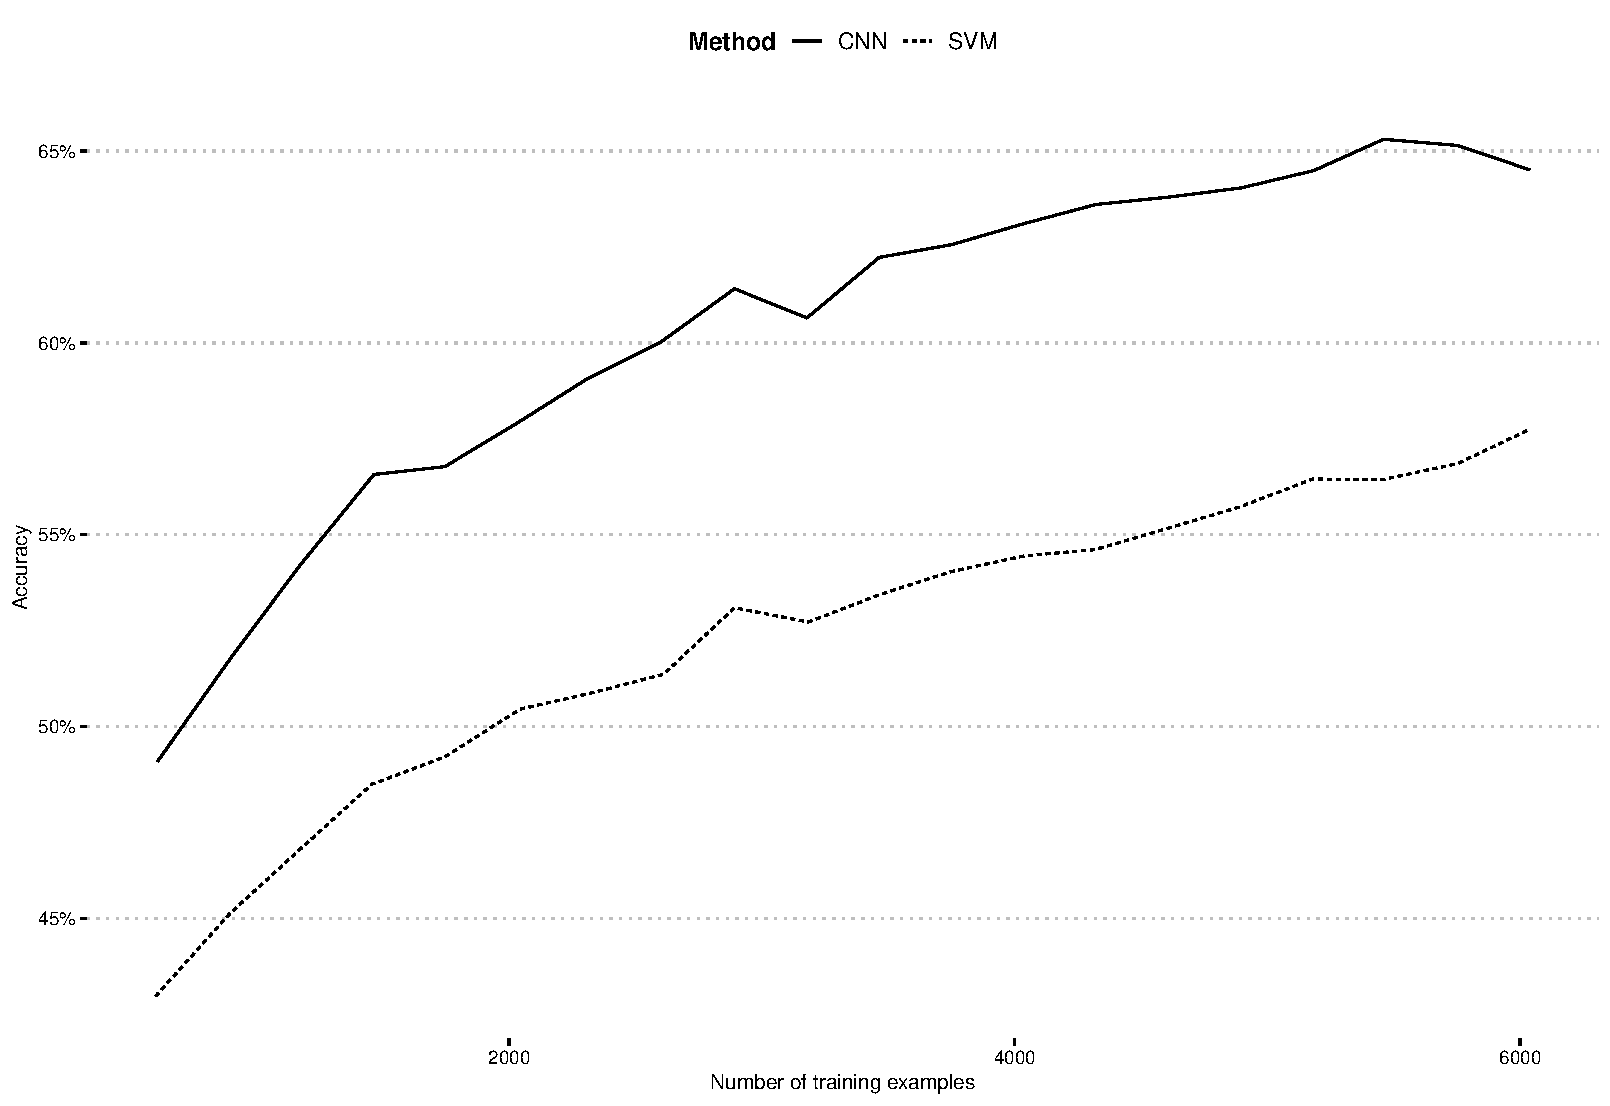
\includegraphics[width=.8\textwidth]{figures/fig_curve.pdf}}

\emph{Note:} Each line shows how quickly more training examples allowed the algorithm to improve performance on the gold standard. For example, with 2000 training documents from the original data of \cite{boukes2019}, the SVM model achieved an accuracy of about 50\%, which increased to almost 55\% with 4000 examples.
\end{figure*}

\noindent Finally, Figure~\ref{fig:curve} shows the so-called `learning curve' of both machine learning algorithms. 
This figure shows the increase of the algorithms' performance as the number of training examples (i.e. more new sentences) increases.
The learning curve was estimated by training on random subsets of the training data and testing against the gold standard,
and gives an indication of how many training documents are needed to achieve a given performance. 
This curve shows that, as expected, both methods improve most quickly at the beginning, signaled by a steep incline, before leveling off to a presumed asymptote, where adding more training examples no longer increases their performance. 
The climbing lines for both algorithms indicate that presumably neither method is saturated yet, assuming the slight downturn at the end of the CNN curve is an anomaly. 
Thus, one can expect that the performance of both methods will profit from more training data.
However, given that both lines are mostly parallel, there is no indication that the performance of the SVM will converge to the performance of the CNN with an equal amount of training data.
%Hence, it seems that CNN is simply the better method for this task. 

%\begin{figure}[t]
%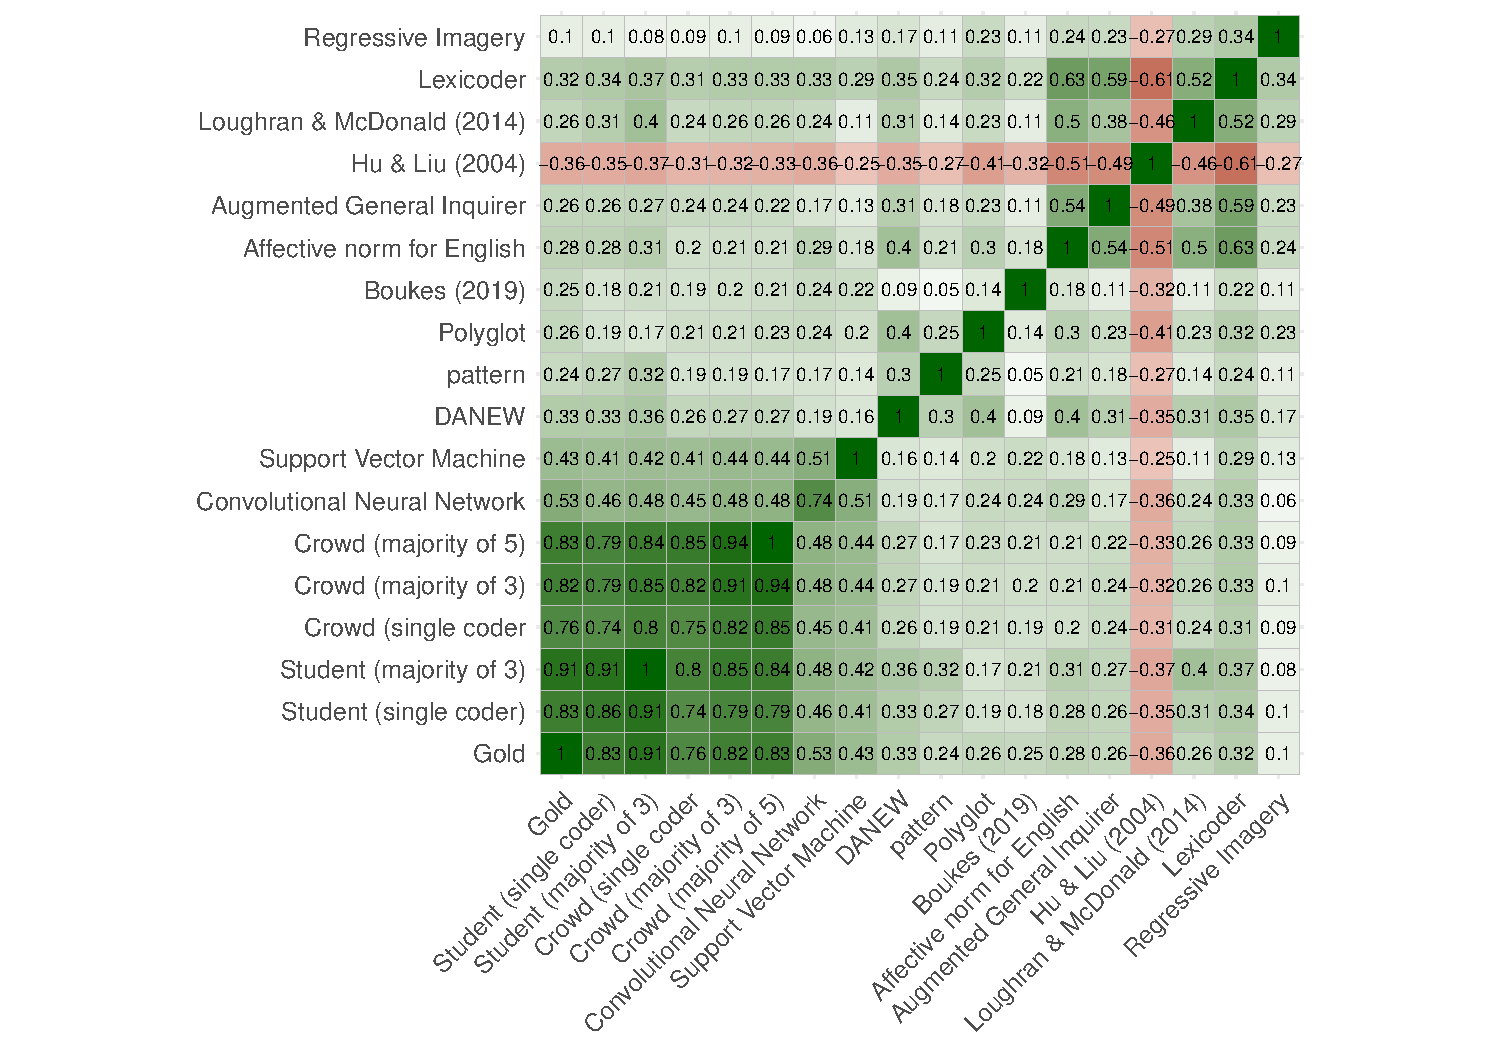
\includegraphics[width=\textwidth]{figures/corr.pdf}
%\caption{Correlation between all methods}\label{fig:corr}
%\textit{Note:} {\small For student and crowd (single coder) and Convolutional Neural Network the average correlation of individual coders/iterations is given. 
%For these methods, diagonal gives the between-coder correlation. }
%\end{figure}

%Figure~\ref{fig:corr} shows the correlation between the various methods. Overall, the methods that correlate weakly with the gold standard also %correlate weakly with each other, showing that there is no systematically different underlying variable that they all measure.
%The only pattern is between the English dictionaries used on the translated headlines, which correlate more strongly with each other than with the gold standard.  

\subsection{Error Analysis}

\newcommand{\fnerroranalysis}{\footnote{%
See `error analysis' in the online appendix at \url{https://github.com/vanatteveldt/ecosent}%
}}

\newcommand{\trans}[2]{\emph{#1} (#2)}

We conducted an error analysis to improve our understanding of the mistakes made by the various automatic methods.\fnerroranalysis{} 
For the error analysis on the off-the-shelf dictionaries, we picked the NRC dictionary, 
the best performing Dutch dictionary (by alpha) that also has an English translation. 
Many of the mistakes made in the Dutch NRC dictionary are missed negations. 
For example positively classifying the word \trans{groei}{growth} in sentences like \trans{afnemende groei hypotheken}{reduced growth in mortgages}  or \trans{matige groei}{tepid growth} or negatively classifying the word \emph{crisis} in \trans{Cyprus heft laatste restricties op na crisis}{Cyprus lifts last restrictions after the crisis}. 
In addition, the error analysis revealed  clear mistakes, such as misclassifying the word \trans{beurs}{stock exchange} as positive. 

The English NRC dictionary applied to headlines translated by deepl shows a similar pattern, with the words \emph{job} and \emph{savings} being misclassified as positive in sentences such as \emph{Best Buy deletes 1500 jobs} and \emph{300 million in savings gone in one day}. The same happened to negative words like \emph{crisis} and \emph{inflation}. 

To better understand the role of translation, we then looked at the sentences that were correctly classified in Dutch but missed by the translated version. An inspection of these ($n=54$) sentences suggests that, although some are translated a bit clumsily, this does not seem to be the cause of the errors as the translation errors are more concerned with function words rather than the sentiment carrying words (for example, \emph{300 million in savings gone in one day} was actually translated as \emph{300 million in savings in one day away}). An interesting detail is that the word \emph{interest} caused most of the translated misclassifications as the English word \emph{interest} is ambiguous between the supposedly neutral meaning of interest rate and the positive concept of being interested or interesting, while the Dutch translation (rente) is not ambiguous. 

For the error analysis of our machine learning approaches, we first look at Naive Bayes as that method has the most interpretable feature weights. Interestingly, the words \trans{faillissement}{bankruptcy} and \trans{werkloosheid}{unemployment} were positive features, presumably because these words are often negated in the training documents. Being based on word frequencies (bag of words), Naive Bayes also suffers from the same lack of context as the dictionaries, for example classifying the sentences \trans{minder woningen onder water}{fewer underwater mortgages} as negative based on negative values for both \emph{fewer} and \emph{underwater}, even though the result of the former is actually to negate the latter. 

The convolutional neural network can take word context into account, but unfortunately the more complex parameters are not easy to inspect manually. When inspecting the misclassified sentences manually, however, it turns out to make some of the same mistakes as the other methods, for example classifying \emph{more bankruptcies} as positive. For many other sentences it is less clear why they are misclassified, although they do seem to have a large amount of rare or new words such as \trans{Werkgevers torpederen caos}{employers torpedo collective-bargaining-agreements}, \trans{dubbelfout bij crisistaks}{double-error with crisis-tax} and \trans{Grieken zijn weer platzak}{Greeks are stone-broke again}. 
Then again, all these words were in the word embeddings and most had sensible synonyms, for example listing \trans{werkgeversheffing}{employer charge} and \trans{graaitax}{grabber tax} as synonyms for \emph{crisistaks}, although \emph{caos} was misclassified 
(presumably due to the failed lemmatization to the singular form \emph{CAO}) and \trans{dubbelfout}{double error} was related mostly to tennis terms. 
Still, since the close synonyms of these rare words are mostly rare words themselves, it is possible that even though the embeddings vectors does words not in the training data to be used for classification, if the words occur in too few contexts in the documents used for creating the embeddings they will still cause difficulties for the algorithm. 




